\documentclass{article}
\usepackage[utf8]{inputenc}

\title{IP Major opdracht 19-20}
\author{Tom Eversdijk \& Wannes Fransen}

\usepackage{natbib}
\usepackage{graphicx}
\graphicspath{ {./img/} }

\usepackage{url}
\usepackage{float}
\usepackage{hyperref}

\begin{document}
\maketitle

\section{Inleiding}
\begin{itemize}
    \item Deadline: \textbf{\date{Woensdag 20 mei 2020, 08u00 CEST}}. 
    \item Je werkt individueel aan de volledige opgave.
    \item Er wordt gebruik gemaakt van een github classroom. Accepteer hiervoor de link op Toledo.
    
    \item Tijdens het examen zul je een extra functionaliteit moeten toevoegen aan je applicatie, zorg er dus voor dat je applicatie eenvoudig uitgebreid kan worden en dat je perfect weet hoe je applicatie werkt. Dit komt bovendien ook van pas tijdens de mondelinge verdediging.
    \item Dit project telt voor 30\% mee voor je uiteindelijke score van dit vak. Deze 30\% geldt enkel voor het project, de uitbereiding die tijdens het examen wordt toegevoegd is onderdeel van de 70\% van het examen.
    \item Omdat het project een onderdeel is voor de evaluatie van dit vak, is het examenreglement hierop van toepassing. Schrijf dus je eigen oplossing! Wanneer je hulp krijgt of geeft aan een mede-student, zorg er dan voor dat het altijd over algemeen advies gaat en deel geen code. Vermeld ook altijd je bron. Dit geldt zowel voor contact in persoon maar ook voor advies via online forums. 
    \item Heb je problemen met je project kun je altijd naar het monitoraat komen. Daarnaast is het ook mogelijk om je vraag op het Toledo forum te plaatsen. Mails met vragen zullen onbeantwoord blijven.
\end{itemize}{}
\section{Opgave}
De opgave is om een applicatie te ontwikkelen waar dat gebruikers informatie kunnen bijhouden welke honden en katten ze zijn tegen gekomen. We willen onthouden wat de naam van het dier was, weten of het een kat of een hond is, wanneer het is geboren en wie dat het baasje is. Daarnaast willen we dat een third party application gebruik kan maken van onze API om  een overzicht te krijgen welke honden en katten we zijn tegengekomen, nieuwe honden en katten kan toevoegen, reeds gekende honden en katten kan wijzigen en zelfs kan verwijderen. Bovendien moet er een onderscheid gemaakt worden tussen een standaard gebruiker die zich aanmeld en een admin. Een admin moet naast de functionaliteiten die een standaard gebruiker heeft, een extra functionaliteit hebben om gebruikers te verwijderen en om het wachtwoord van een gebruiker aan te passen.

\section{API}
Met de API is het de bedoeling dat een third party application honden en katten kan toevoegen, reeds gekende honden en katten kan wijzigen en bestaande honden en katten kan verwijderen \textbf{die van jou zijn}. Om een van deze acties uit te kunnen voeren moet in de https requests header een geldige API key meegegeven worden. Bovendien is het de bedoeling om voor iedere third party application een nieuwe API key mee te geven. Zo kunnen we eenvoudig de toegang van 1 third party application blokkeren door het intrekken van overeenkomstige API key.
\\
\\
De API key bestaat uit een random string zonder verlooptijd (string mag zelf gegenereerd worden). Er hoeft geen signing van deze random string te gebeuren en sla deze string mee op in je database. De token word doorgestuurd met volgende header-key "MyFancyHeader:$<$API-key$>$".
Het gemakkelijkste om deze token te verwerken is om een plug te schrijven die uit de request de nodige request headers haalt en deze verwerkt. Door middel van de Plug.Conn kan dit eenvoudig bereikt worden. \url{https://hexdocs.pm/plug/Plug.Conn.html}

\subsection{Create}
Voorzie een API endpoint om door middel van een POST request een dier toe te voegen.

\subsection{Read (overview)}
Voorzie een API endpoint om door middel van een GET request alle dieren (beperkt) te tonen. \textbf{LET OP: Dit zijn enkel jouw dieren} Voorbeeld output zou zijn:

\begin{verbatim}
[
    {
        "id": 1,
        "name": "snuffles"
    },
    {
        "id": 2,
        "name": "wuffles"
    }
]
\end{verbatim}

\subsection{Read (animal details)}
Voorzie een API endpoint om door middel van een GET request info over een specifiek dier op te vragen. Voorbeeld output zou zijn:

\begin{verbatim}
{
    "id": 1,
    "name": "snuffles",
    "dob": "...",
    "cat_or_dog": "hybrid"
}
\end{verbatim}


\subsection{Update}
Voorzie een API endpoint om door middel van een PUT of PATCH request een dier up te daten op basis van ID.

\subsection{Delete}
Voorzie een API endpoint om door middel van een DELETE request een dier te verwijderen op basis van ID.

\subsection{EXTRA}
Je kan enkel je eigen dieren beheren door middel van API keys. Bij het binnenkomen v.e. request, ga je nakijken of de meegegeven API key geldig is voor de gebruiker van wie je dieren wilt aanpassen/lezen.

\section{Pagina's}
Om de opgave tot een goed einde te brengen is het nodig om verschillende pagina's met hun eigen functionaliteit te ontwerpen. In deze sectie wordt er dieper ingegaan op de verwachtingen van iedere pagina.

\subsection{Header}
Met uitzondering van de login pagina [\ref{subsect:login_pagina}] en de raw-api [\ref{subsect:raw_api}] pagina wordt er verwacht dat iedere volgende pagina gebruik maakt van eenzelfde header. Deze header wordt gebruikt door de gebruiker om zichzelf te kunnen navigeren tussen de verschillende paginas. Meer concreet moet de header de volgende functionaliteiten bevatten: Veranderen van taal (minstens 2 verschillende talen), uitloggen uit de applicatie,  navigeren naar de show profile [\ref{subsect:show_profile}] pagina en terug navigeren naar de home pagina [\ref{subsect:home_page}]. Voor een admin gebruiker moet het ook mogelijk zijn om naar de user management pagina [\ref{subsect: user management}] te gaan.

\subsection{Login pagina} 
\label{subsect:login_pagina}
Zoals de naam als doet vermoeden is dit de pagina waar dat een gebruiker kan inloggen. Het inloggen gebeurd op basis van een gebruikersnaam \& wachtwoord. Door op de sign up knop te drukken word je doorverwezen naar een sign up pagina waardat niewe gebruikers zicht kunnen registreren. 

\subsection{Sign up pagina}
Op deze pagina kan een nieuwe gebruiker zichzelf registreren. Het aanmaken van een account kan door het geven van een gebruikersnaam en een wachtwoord. Controlleer ook zeken of dat de gebruikersnaam uniek is. Voor het opslaan van het wachtwoord mag Pbkdf2 gebruikt worden als hash algoritme. \\

Authenticatie is d.m.v. JWT, dus geen sessions!

\subsection{Dashboard} 
\label{subsect:home_page}
Het dashboard is de pagina waar dat de gebruik op terecht zal komen nadat deze zichzelf heeft aangemeld. Hier wordt een overzicht gegeven van al de honden en katten van de gebruiker. Daarnaast moet de gebruiker door middel van javascript kunnen zien hoe laat het op dit moment is. \\

\textit{Via de browser is het \textbf{nergens} mogelijk om katten / honden te kunnen aanmaken /aanpassen / verwijderen, \textbf{wel via REST.}}

\subsection{Show profile}
\label{subsect:show_profile}
Op deze pagina wordt er verwacht dat een gebruiker zijn eigen gebruikersnaam kan zien. Naast het zien van de eigen gebruikersnaam bevat deze pagina een knop om verder te gaan naar de edit profile[\ref{subsect:Edit_profile}] pagina en een knop om de gebruiker zijn wachtwoord te laten veranderen[\ref{subsect:change_password}]. \\

Daarnaast wordt er verwacht dat de gebruiker op deze pagina al zijn API-keys met de bijhorende naam kan zien [\ref{subsect:raw_api}], verwijderen en nieuwe API-keys kan genereren met een gegeven naam.
% TODO: aanpassen image

\subsection{Edit username}
\label{subsect:Edit_profile}
De enige functionaliteit van deze pagina bestaat eruit dat een gebruiker zijn gebruikersnaam kan wijzigen. Zodra de gebruikersnaam is gewijzigd moet de gebruiker in staat zijn om met zijn gewijzigde gebruikersnaam in te loggen op de applicatie.

\subsection{Change password}
\label{subsect:change_password}
Deze pagina bevat de mogelijkheid om het wachtwoord van een gebruiker aan te passen. Om veiligheidsredenen wordt er verwacht dat de gebruiker zijn vorig wachtwoord nodig heeft om een nieuw wachtwoord in te stellen. Bovendien moet het nieuw wachtwoord twee maal ingevoerd worden om de kans op typefouten te minimaliseren.


\subsection{API key displayen (raw text)}
\label{subsect:raw_api}
Deze pagina bevat geen layout, het enige wat er op deze pagina zichtbaar moet zijn is de API key van de geselecteerde key in de show profile pagina[\ref{subsect:show_profile}].


\subsection{User management}
\label{subsect: user management}
Deze pagina is alleen beschikbaar als een admin zich heeft aangemeld. Er wordt een overzicht gegevens van al de gebruikers. Om het eenvoudig te houden is het de admin zelf die een nieuw wachtwoord voor een gebruiker kiest. \\

Per opgelijste user, zie je de knoppen 
\begin{itemize}
    \item Edit
    \item Delete
\end{itemize}


\subsubsection{Edit user page}
Op deze pagina kan een admin de gebruikersnaam \& wachtwoord van een gebruiker wijzigen. Er is een save button en een cancel button om terug naar het overzicht te gaan.



\pagebreak

\section{Images}

\begin{figure}[!h]
    \centering
    \includegraphics{login_page}
    \caption{Login page}
    \label{fig:login page}
\end{figure}

\begin{figure}[!h]
	\centering
	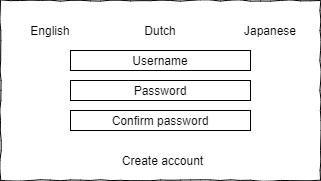
\includegraphics{createUser}
	\caption{Sign up page}
	\label{fig:create user page}
\end{figure}

\begin{figure}[!h]
    \centering
    \includegraphics{Header}
    \caption{Header}
    \label{fig:header}
\end{figure}

\begin{figure}[!h]
    \centering
    \includegraphics{home_page}
    \caption{Home page}
    \label{fig:home page}
\end{figure}

\begin{figure}[!h]
    \centering
    \includegraphics{show_profile}
    \caption{Show profile}
    \label{fig:show_profile}
\end{figure}

\begin{figure}[!h]
    \centering
    \includegraphics{edit_user}
    \caption{edit user}
    \label{fig:edit profile}
\end{figure}

\begin{figure}[!h]
    \centering
    \includegraphics{change_password}
    \caption{Change password}
    \label{fig:Change password}
\end{figure}

\begin{figure}[!h]
    \centering
    \includegraphics{api}
    \caption{Raw api}
    \label{fig:raw api}
\end{figure}

\begin{figure}[!h]
    \centering
    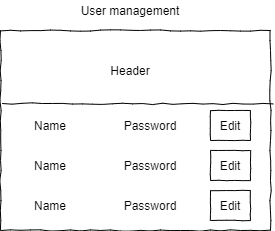
\includegraphics{user_management}
    \caption{user management}
    \label{fig:user management}
\end{figure}

\begin{figure}[!h]
    \centering
    \includegraphics{usr_management_edit}
    \caption{User edit as admin}
    \label{fig:usr_management_edit}
\end{figure}



\end{document}